\documentclass[12pt,a4paper]{report}
\usepackage{graphicx}
\usepackage{amsmath}
\usepackage{fancyhdr}
\usepackage{cite}
\usepackage{a4wide}
\usepackage{float}
\usepackage{epsfig}
\usepackage{longtable}
\usepackage{enumerate}
\usepackage{afterpage}
\usepackage{multirow}
\usepackage{ragged2e}
\usepackage{gensymb}
\usepackage{amsfonts} 
\usepackage[left=3.5cm,top=1.5cm,right=3cm,bottom=3cm]{geometry}
\usepackage{setspace}           
\usepackage{float}
\usepackage{txfonts}
\usepackage{lipsum}
\usepackage{tikz}
\usetikzlibrary{calc}
\usepackage{subfiles} % Best loaded last in the preamble


\newcommand{\Usefont}[1]{\fontfamily{#1}\selectfont}

\usepackage{lscape} % for landscape tables
\renewcommand{\baselinestretch}{1.7} 

\usepackage{blindtext}
\usepackage{xpatch}
\usepackage{url}
\usepackage{leqno}
\usepackage{subcaption}

\linespread{1.5}
\usepackage[intoc, english]{nomencl}
\hyphenpenalty=5000
\tolerance=1000
\usepackage[nottoc]{tocbibind}
\bibliographystyle{IEEEtran}
\renewcommand{\bibname}{References}

%********************************************************
%*********************Figures*****************************
% Save all figures in the folder figures and include them in your 
% report using the command \includegraphics{figure-name}

\graphicspath{{figures/}}

% figure files can be in jpeg,jpg, png or pdf formats
%*******************************************************************


\begin{document}
	
	
%****The entries in this section are to be filled in by the student with appropriate values *************

% These values are used thorough out the report 
% please fill in the appropriate values

\gdef \title{Epileptic Seizure Detection in EEG Signal Using Machine Learning and Deep Learning Techniques } % Seminar title
\gdef \author{ALJO K J}	 %student name
\gdef \rollno{KNP22CS024} %KTU Reg No
\gdef \acadyear{2025-26} % Academic year
\gdef \month{September 2025} %Month of Report submission
\gdef \date{08-09-2025} %Date of signing the declaration
\gdef \dept{Computer Science and Engineering} %Department
\gdef \deptabbr{Dept.of CS} %Dept name abbreviation
\gdef \degree{Bachelor of Technology} %degree
\gdef \branch{Computer Science and  Engineering} %branch
\gdef \college{College of Engineering Karunagappally}
\gdef \collegeplace{Kollam}
\gdef \collegetown{Karunagappally}

\gdef \guide{Shabana A S} %Seminar guide
\gdef \guidedes{Assistant Professor}%Seminar guide designation
\gdef \semcordinatorA{Jyothi Vijayan } % Seminar coordinator 2 
\gdef \semcordinatorAdes{Assistant Professor}% Seminar coordinator 2 designation


\gdef \hod{Dr. Smitha P} %Head of Department
\gdef \hoddes{Professor and Head} %HOD designation
%*******************************************************************
% The font pages. The source tex files are there in the folder
%==================================coverpage.tex================================


\newenvironment{coverpage}
\thispagestyle{empty}
\begin{titlepage}
\subfile{design_cover}
	\begin{center}
		{\Usefont{phv} \Large \bf \title \par}
		\vspace*{10pt}
		\large \em \Usefont{pzc}{ 
			A Seminar Report \par
			Submitted to the APJ Abdul Kalam Technological University\\
			in partial fulfillment of requirements for the award of degree}\\ [.15\baselineskip] \par
		\Usefont{ppl} {\bfseries  \degree}\\
		in\\
		{\Usefont{ppl} {\bfseries \branch}}\\
		by\\
		\bf {\author}\\
		\bf{\rollno}
		\vspace*{20pt}
		\centering
		\begin{figure}[h!]
			\centerline{
\includegraphics[scale=0.5]{cek-logo.png}}
		\end{figure}
		
		\vspace{\stretch{0.5}}
		\small{\bf DEPARTMENT OF COMPUTER SCIENCE AND  ENGINEERING} \par
		\bf{COLLEGE OF ENGINEERING KARUNAGAPPALLY} \par
		\bf{KERALA} \par
		\bf{\month}
	\end{center}
\end{titlepage}	
 %Unless essential Do not edit this tex file



%%********************Certificate*******************

% To print name of only the seminar coordinator 1 in the certificate page
%==================================certificate1.tex================================
% To print name of only the seminar coordinator 1 in the certificate page

\newenvironment{certificate1}

	\newpage
	\begin{center}	
		%\vspace{1.5cm}
		
		\textbf{DEPARTMENT OF COMPUTER SCIENCE AND  ENGINEERING}\\	
		\textbf{COLLEGE OF ENGINEERING KARUNAGAPPALLY}	
		
		
		\textbf{\acadyear} 
	\end{center}
	
	\begin{center}
		
\includegraphics[scale=0.5]{cek-logo.png}	
	\end{center}
	\begin{center}
		\textbf{CERTIFICATE}
	\end{center}
	
	This is to certify that the report entitled \textbf{\title} submitted by \textbf{\author}\hspace*{2pt}(\rollno), to Department of \branch in partial fulfillment of the B.Tech.\ degree in \textbf{\branch}\hspace*{2pt} is a bonafide record of the seminar work carried out by him under our guidance and supervision. This report in any form has not been submitted to any other University or Institute for any purpose.
	
	
	\begin{singlespace}
		\vspace*{2cm}
		\begin{table}[h!]
			\centering
			\begin{tabular}{p{7cm} p{1.5cm} p{7cm}} 
				\textbf{\guide} && \textbf{\semcordinatorA} \\
				(Seminar Guide) &&  (Seminar Coordinator)\\
				\guidedes & & \semcordinatorAdes\\ 
				Dept.of CSE && Dept.of CSE\\ 
				College of Engineering && College of Engineering \\
				Karunagappally && Karunagappally\\
			\end{tabular}
			
		\end{table}
		
		\vspace*{1.3cm}
		
		\begin{center}
			
% 			\hline
			\textbf{\hod} \\ 
			\hoddes\\ 
			Dept.of CSE\\ 
			College of Engineering\\
			Karunagappally\\
			
		\end{center}
	\end{singlespace}
	
	\thispagestyle{empty}



 

% To print names of both the seminar coordinators in the certificate page
%\include{certificate2} %Please uncomment this and comment the previous line

%%***************************************************


%==================================declaration.tex================================
%
\newpage
\newenvironment{declaration}
\thispagestyle{empty}
\begin{center}
\vspace*{50pt}
\textbf{DECLARATION}\\
\end{center}
I \author \hspace*{2pt} hereby declare that the seminar report {\bf{\title}}, submitted for partial fulfillment of the requirements for the award of degree of Bachelor of Technology of the APJ Abdul Kalam Technological University,Kerala is a bonafide work done by me under supervision of \guide \hspace*{2pt}. \par
This submission represents my ideas in my own words and where ideas or words of others have been included, I have adequately and accurately cited and referenced the original sources.\par 
I also declare that I have adhered to ethics of academic honesty and integrity and have not misrepresented or fabricated any data or idea or fact or source in my submission. I understand that any violation of the above will be a cause for disciplinary action by the institute and/or the
University and can also evoke penal action from the sources which have thus not been properly cited or from whom proper permission has not been obtained. This report has not been previously formed the basis for the award of any degree, diploma or similar title of any other University.

\noindent \begin{minipage}{0.45\linewidth}
\begin{flushleft}
\vspace{2.5cm}

\collegetown \\
\date

\end{flushleft} 
\end{minipage}
\hfill
\begin{minipage}{0.45\linewidth}
\begin{flushright}                                      
\vspace{1.5cm}

\author\\


\end{flushright} 
\end{minipage}
\thispagestyle{empty}
 %Unless essential Do not edit this tex file

\pagenumbering{roman} 

%%********************************Abstract***********************
%============================= abstract.tex================================
\chapter*{Abstract}%
%\addcontentsline{toc}{chapter}{\numberline{}Abstract}%
\addcontentsline{toc}{chapter}{Abstract}%

This research presents a novel approach to detecting epileptic seizures leveraging the strengths of Machine Learning (ML) and Deep Learning (DL) algorithms in EEG signals. Epileptic seizures are neurological events with distinctive features found in Electroencephalography (EEG) that lend considerable credibility to researchers. Machine Learning (ML) and Deep learning (DL) algorithms have emerged as powerful feature extraction and classification tools in EEG signal analysis. Many studies have converted the EEG signals into either images and /or calculated time-frequency domain features and performed classification. This study focuses on classifying time-series data representation of EEG signals with machine learning-based classifiers by tuning parameters and deep learning-based One-Dimensional Convolutional Neural Network (1D CNN) methods. The primary objective is not only to determine the optimal classifier but also to emphasize critical metrics such as sensitivity, precision, and accuracy, which are critical in medical investigations, particularly for the early detection of diseases and patient care optimization. The UCI Epileptic Seizure Recognition dataset used in this study consists of time-series data points extracted from the EEG signals. The dataset has been preprocessed and fed to the classifiers, namely Extreme Gradient Boosting (XGBoost), TabNet, Random Forest (RF), One Dimensional Convolutional Neural Network, and achieved encouraging accuracies of 98\%, 96\%, 98\%, and 99\%, respectively. The proposed 1D-CNN model performed better than other state-of-the-art models concerning accuracy, sensitivity, precision, and recall. \\


\thispagestyle{plain}
%=======================================================================

 % Please type in the abstract in this tex file abstract.tex

%%***************************************************
% Default Acknowledgement page
%==================================acknowledgement.tex=============================
\chapter*{Acknowledgement}%
\addcontentsline{toc}{chapter}{Acknowledgement}%

%\newenvironment{acknowledgement}

I take this opportunity to express my deepest gratitude and sincere thanks to everyone who helped me to complete this work successfully. I express my sincere thanks to Dr. Smitha Dharan, Principal, College Of Engineering Karunagappally, Kollam and \hod, Head of Department, \dept, \college\hspace*{2pt} \collegeplace, \hspace*{2pt} for providing  me with all the necessary facilities and support.I would like to express my sincere gratitude to \guide, \hspace*{2pt}department of \hspace*{2pt} \dept, \hspace*{2pt} \college, \hspace*{2pt} \collegeplace \hspace*{2pt} for their support and co-operation.I would like to place on record my sincere gratitude to my seminar guide \guide,\hspace*{2pt}\guidedes,\hspace*{2pt}\dept,\hspace*{2pt}\college \hspace*{2pt}, Kollam for the guidance and mentorship throughout the course.Finally I thank my family, and friends who contributed to the succesful fulfilment of this seminar work.

\vspace*{30pt}
\begin{flushright}
	\textbf{\author}
\end{flushright}
\thispagestyle{plain}
  %Unless essential Do not edit this tex file


%%***************************************************
%%**If you have only one seminar coordinator faculty member
% please comment the above line and uncomment this line

%\include{acknowledgement1}  %Unless essential Do not edit this tex file
%*******************************************************************

\thispagestyle{empty}
\newpage
    
%%**********************Table of Contents***********************
\tableofcontents
\listoffigures
\listoftables
 %List of Symbols (Optional) comment if not required.
% symbold may be added in the file symbol.tex

%%********************Body of the report**********
% Arabic numbering is used in the body of the report

\cleardoublepage
\setcounter{page}{1}
\pagenumbering{arabic}


%%********************Chapter 1**********
\chapter[Introduction]{\Huge Introduction}
Epilepsy represents one of the most prevalent neurological disorders worldwide, affecting approximately 50 million individuals globally according to the World Health Organization. This chronic condition is characterized by recurrent and unpredictable seizures that significantly impact the quality of life for affected individuals. Epileptic seizures manifest as sudden and temporary disturbances in normal brain functioning, resulting from abnormal and excessive electrical activity in neurons. These electrical disruptions can lead to various physical and mental manifestations, ranging from subtle sensations to severe convulsions and loss of consciousness, sometimes even resulting in sudden unexpected death.
The accurate detection and diagnosis of epileptic seizures is crucial for developing effective treatment strategies and ensuring optimal patient care. Traditional methods of seizure detection rely heavily on manual interpretation of electroencephalography (EEG) signals, which record the electrical activity of the brain through electrodes placed on the scalp. However, manual EEG analysis is time-consuming, requires specialized expertise, and may be subject to human error and variability in interpretation.
\section{Background and Motivation}
Recent advances in computational technologies have opened new avenues for automated seizure detection systems. Machine Learning (ML) and Deep Learning (DL) algorithms have emerged as powerful tools for pattern recognition and classification in biomedical signal processing. These techniques offer the potential to overcome the limitations of traditional manual interpretation by providing consistent, automated analysis of EEG signals with high accuracy and reliability.
The motivation for this research stems from the critical need for reliable, automated epileptic seizure detection systems that can assist healthcare professionals in making timely and accurate diagnoses. While existing studies have achieved notable results in seizure classification, there remains a gap in comprehensive evaluation using multiple metrics that are essential for medical applications, particularly sensitivity, precision, and recall alongside accuracy.

\section{Problem Statement}
Current automated seizure detection systems face challenges including EEG signal complexity, inter-patient variability, and computational efficiency requirements. Many existing approaches focus primarily on classification accuracy without adequate emphasis on critical medical metrics such as sensitivity and precision that are essential for clinical deployment. The challenge lies in developing robust classification systems that can effectively distinguish between seizure and non-seizure patterns while maintaining high performance across multiple evaluation metrics.

\section{Objectives of the Seminar}
The primary objective is to present a comparative approach to epileptic seizure detection using optimized machine learning and deep learning classifiers including XGBoost, TabNet, Random Forest, and 1D CNN on time-series EEG data. The study aims to emphasize comprehensive medical metrics beyond accuracy, specifically sensitivity, precision, recall, and F1-score, which are crucial for medical applications and clinical decision-making.

\section{Organization of the Report}
This report is structured into six chapters for clarity and coherence. Chapter 2 presents a detailed literature review and surveys major contributions and related work in the field of epileptic seizure detection using machine learning and deep learning techniques. Chapter 3 introduces the proposed methodology by explaining the dataset description, preprocessing approaches, and the implementation details of XGBoost, TabNet, Random Forest, and 1D CNN classifiers used in this study.Chapter 4 discusses the performance evaluation and results with comprehensive analysis using multiple evaluation metrics including accuracy, precision, recall, F1-score, ROC-AUC curves, confusion matrices, and additional metrics such as CSI, MCC, and Cohen's Kappa. Chapter 5 outlines the advantages of the proposed approach, highlighting the superior performance in terms of medical metrics and comparative analysis with existing state-of-the-art methods. Finally, Chapter 6 concludes the report by summarizing the key findings, discussing limitations and challenges encountered, and outlining potential avenues for future research in automated epileptic seizure detection systems.



%%********************Chapter 2**********
\chapter{Literature Review}
The research on epileptic seizure detection in EEG signals has spanned a variety of machine learning and deep learning techniques. While significant progress has been made, most approaches remain fragmented, focusing on isolated technical aspects without converging into a unified and comprehensive framework. This section critically examines notable contributions, analyzing both their strengths and shortcomings.

[1] A. Dogra et al. investigated epileptic seizure detection by employing the discrete wavelet transform (DWT) to extract the intricate frequency components inherent in EEG signals. This method quantifies the energy within specific frequency bands at particular times within a signal. Their approach utilizes an optimized k-nearest neighbors (KNN) algorithm for enhanced detection accuracy.

[2] Y. Kaya et al. extracted quantitative features from EEG data using a one-dimensional local binary pattern (IDLBP). This is a texture operator that labels the pixels of an image by thresholding the neighborhood of each pixel and considering the result as a binary number. These features were then fed to various classifiers, including logistic regression, BayesNet, and SVM.

[3] M. Mursalin et al. introduced an innovative approach to identifying epileptic seizures by using the Improved Correlation-based Feature Selection (ICFS) method in conjunction with a Random Forest (RF) classifier. This methodology entails an initial step of employing ICFS to extract key features from the time, frequency, and entropy domains. ICFS is a feature selection technique that selects subsets of features that are highly correlated with the target variable but have low correlation with each other.

Deep learning techniques have also been widely utilized for their ability to autonomously extract features from raw EEG data. A study by [4] N. K. C. Pratiwi et al. proposed a 1D-CNN approach by converting EEG signals into 2D/3D images, achieving 96.30\% accuracy. 

[5] A. Abdelhameed and M. Bayoumi proposed a supervised deep convolutional autoencoder (SDCAE) model to detect seizures in children, achieving an accuracy of 98.79\%. An autoencoder is a type of neural network that learns to compress input data into a lower-dimensional representation and then reconstruct it. 

[6] I. Ahmad et al. used a hybrid deep learning approach with a 1D-CNN-BILSTM+TBPTT model and achieved a 99.41\% accuracy.

While many studies have achieved high accuracy, the literature review suggests a gap in the lack of emphasis on crucial medical metrics beyond accuracy, such as sensitivity, precision, and recall. The research in the provided document aims to fill this gap by not only developing an effective classifier but also by providing a comprehensive evaluation framework that highlights these crucial metrics.
% Please comment this line and type in the results chapter
	


%%********************Chapter 4**********
\chapter{Proposed Methodology}
This chapter describes the dataset and methods we propose to detect epileptic seizures, including the machine learning algorithms such as extreme gradient boosting classifier (XGBoost), TabNet classifier, Random Forest classifier with fine-tuning their parameters, and a 1D- CNN based deep learning algorithm.
\section{DataSet Description}
UCI Epileptic Seizure Recognition dataset, which is a processed version of the original Bonn dataset. The original Bonn dataset contained EEG signals from five individuals, with each having 100 files of brain activity over 23.6 seconds, with each time series sampled into 4097 data points.




To create the UCI dataset, the 4097 data points were partitioned into 23 segments, each containing 178 data points that represent a 1-second time interval. This was done for all 500 individuals, resulting in 11,500 total data instances for classification purposes.


The dataset has five classes of EEG activity:


Class 1: Seizure activity recordings.


Class 2: EEG signals from the tumor region.


Class 3: EEG recordings from a healthy brain area.


Class 4: EEG recordings taken with eyes closed.


Class 5: EEG recordings taken with eyes open.

For the purpose of this study, a binary classification approach was adopted. The non-seizure classes (2, 3, 4, and 5) were all set to a label of 0, while the seizure class (1) was set to 1. The dataset was then divided into an 80\% training set and a 20\% validation set to ensure data quality and consistency before model training. The EEG signal's variation at different instances can be seen in the figure below.

\begin{figure}[H]
    \centering
    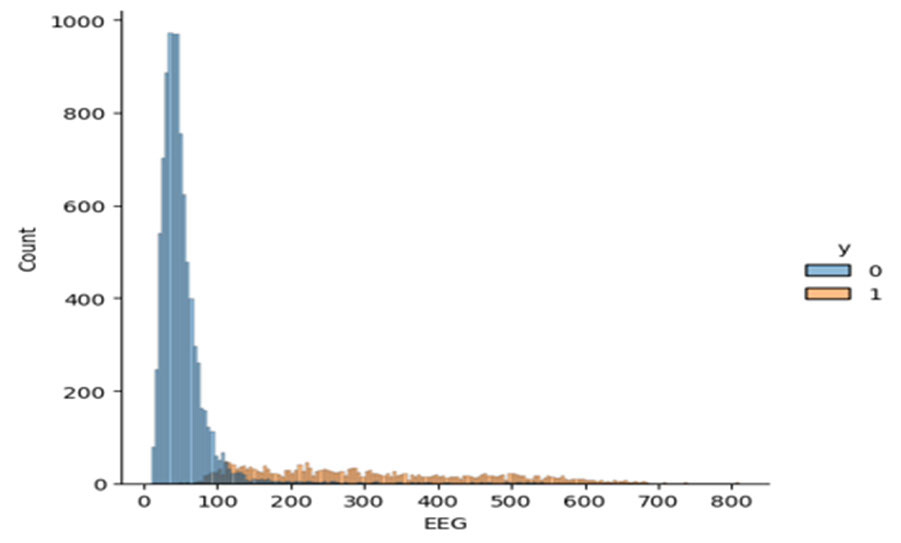
\includegraphics[width=0.8\linewidth]{Images/Figure 2.png}
    \caption{Histogram representation of the epileptic and non-epileptic
seizures in the dataset.}
    \label{fig:eeg_variation}
\end{figure}

\section{Proposed Approach}
This study employs a comprehensive approach utilizing four distinct classifiers: XGBoost, TabNet, decision tree, and 1D-Convolutional Neural Network (CNN). Before model
training, the dataset underwent preprocessing steps to ensure data quality and consistency. The dataset was strategically divided into an 80\% training set and a 20\% validation set.

Figure 3.2 illustrates the framework of the proposed methodology representing data processing, classifiers, and a set of evaluation metrics employed in the approach. In the feature extraction process, Q.Wu and E. Fokoue [7] extracted data points from the EEG signals. In our study, we considered those extracted datapoints as features and further preprocessed and normalized to ensure all the features are on a consistent
scale, preventing certain features from dominating others in the learning process. Further, the data was fed to the classifiers and evaluated with the following metrics as shown in Figure 3.2. 

\begin{figure}[H]
    \centering
    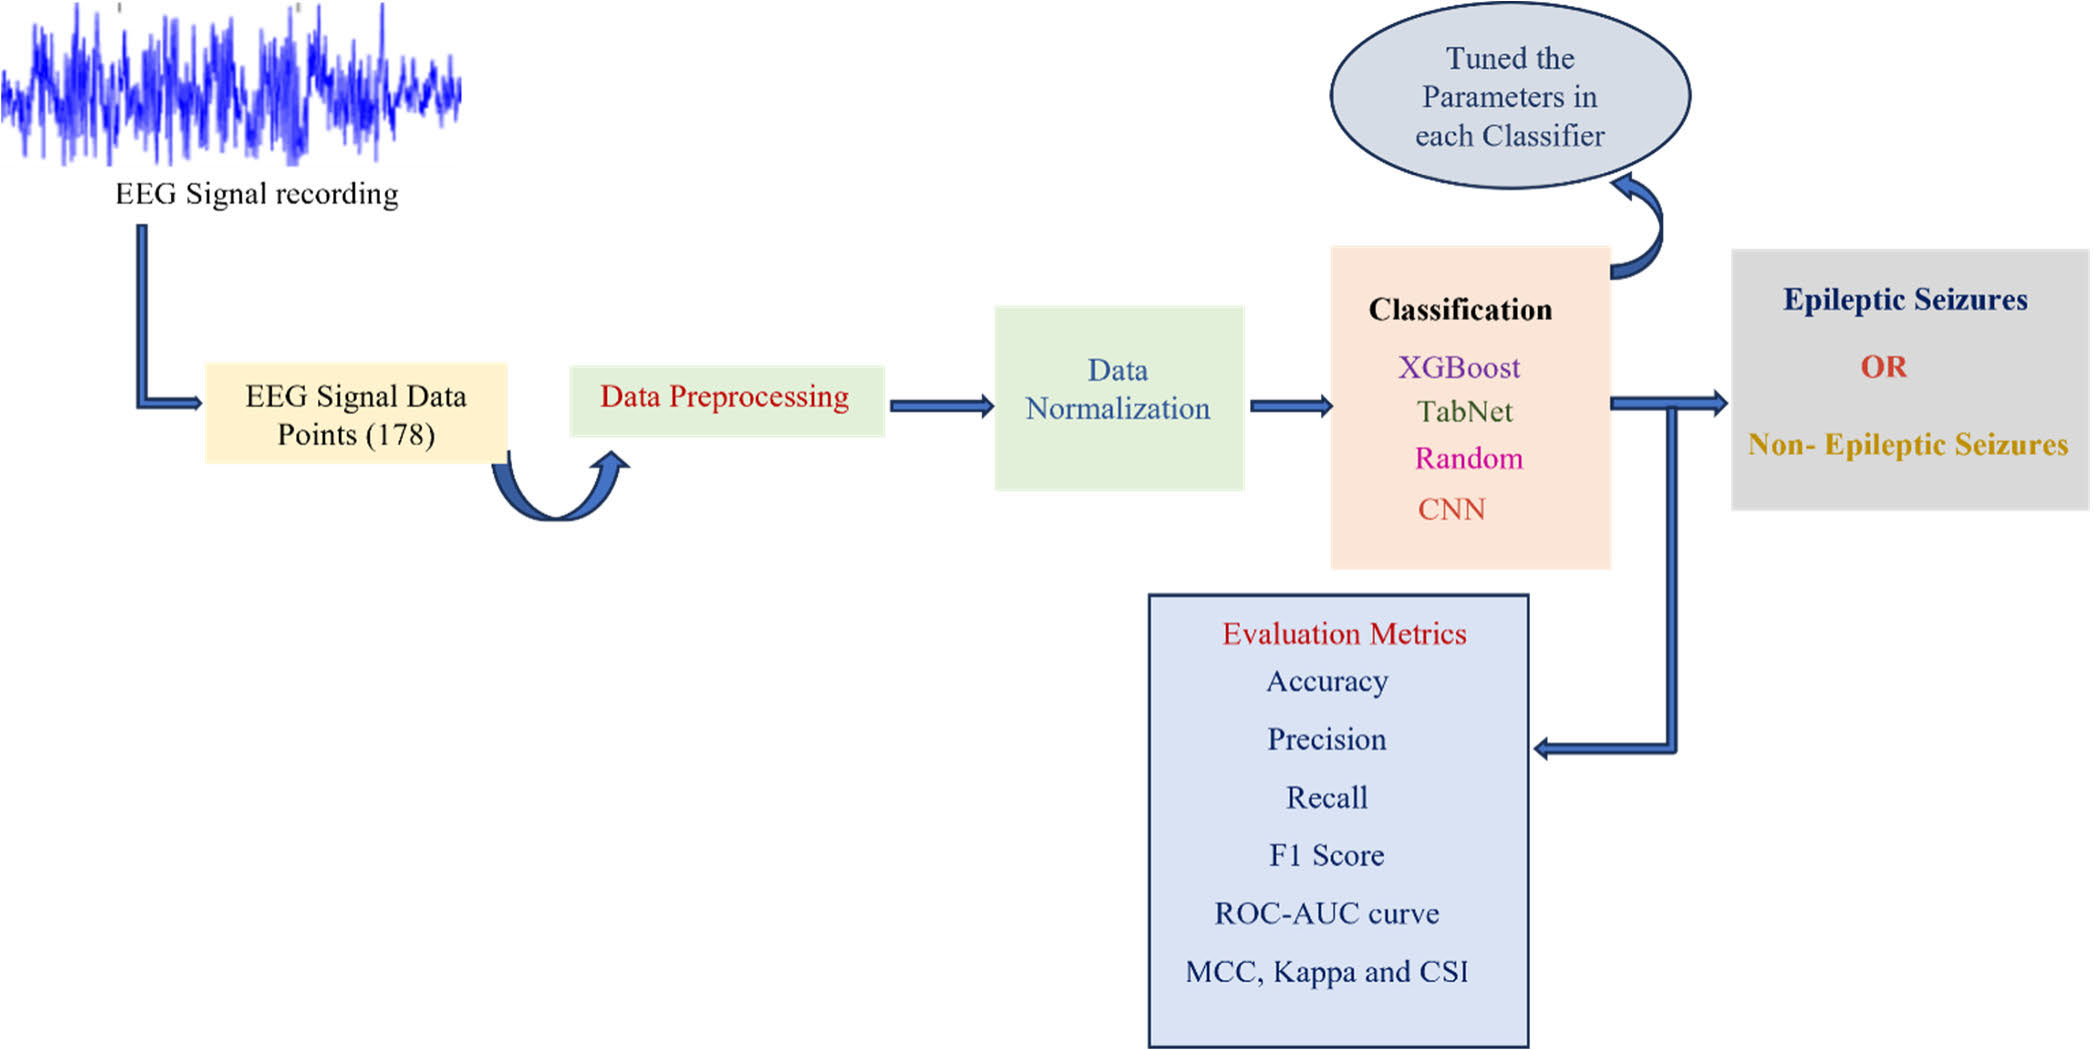
\includegraphics[width=1\linewidth]{Images/Figure 3.png}
    \caption{The Block diagram for the proposed method.}
    \label{fig:proposed_method_blockdiagram}
\end{figure}

\section{XGBoost Classifier}
Extreme Gradient Boosting (XGBoost) [8] is a robust algorithm widely applied in gradient boosting frameworks, effective at capturing temporal dependencies in time-series data through its ensemble of decision trees. This makes it suitable for epileptic seizure detection, where non-linear and complex patterns are common. Its built-in regularization also prevents overfitting, an important factor when handling noisy or outlier-prone data.

For this study, XGBoost was configured as follows: the learning rate was set to 0.01, ensuring a cautious and stable learning process; the regularization parameter ‘alpha’ was applied to reduce the risk of fitting noise; and the booster ‘gbtree’ was chosen for its ability to capture non-linear and temporal relationships. The maximum depth of trees was fixed at 8, allowing the model to learn intricate seizure patterns, while 1000 estimators were used to build a large and diverse ensemble for improved detection performance.

\section{TabNet Classifier}
Tabular Neural Network (TabNet) [9] is a deep learning architecture designed for tabular data with sequential dependencies. Its attention mechanism helps the model focus on relevant time steps, making it effective for epileptic seizure detection where observation order is important. The attention feature also improves interpretability by highlighting which time steps contribute most to classification.

In this study, TabNet was implemented using PyTorch with patience set to 20 and max\_epochs to 100. These parameters enable early stopping, allowing training to halt when validation performance stops improving, thereby reducing overfitting and saving computation

\section{Random Forest Classifier}
Random Forest is an ensemble method that builds multiple decision trees and outputs the majority class, offering high predictive accuracy, robustness to overfitting, and strong performance on high-dimensional data. By combining trees, it generalizes well to different temporal patterns in epileptic seizures and can highlight important features contributing to seizure occurrences.

In this study, Random Forest was configured with 1000 estimators to ensure a large and stable ensemble, random\_state set to 42 for reproducibility, and the ‘gini’ criterion to measure split quality by evaluating misclassification probability.

\section{Convolutional Neural Network (CNN) }
Convolutional Neural Networks (CNNs) are not limited to image data; they can also process sequential data such as EEG time series using one-dimensional (1D) convolutions. In this study, a 1D CNN was implemented with a kernel\_size = 2 to capture short-term features. A max pooling layer was applied to reduce the data dimensions, while the ReLU activation function was used to learn non-linear relationships.  

The architecture consisted of four convolutional layers with filters of 32, 32, 64, and 128, enabling hierarchical feature learning where deeper layers extract higher-level representations. Dropout regularization was used to prevent overfitting, with a rate of 0.2 in the convolutional layers and 0.5 in the fully connected (FC) layer.  

The first FC layer contained 64 neurons with ReLU activation, followed by a final FC layer with one neuron and the Sigmoid activation for binary classification. Training was performed using the Adam optimizer (learning\_rate = 0.0005) with binary cross-entropy as the loss function.  

The functions used are defined as follows:

\begin{equation}
\text{Sigmoid}(x) = \frac{1}{1 + e^{-x}}
\end{equation}

\begin{equation}
\text{ReLU}(x) = \max(0, x)
\end{equation}

\begin{equation}
L(y, \hat{y}) = -\Big[ y \cdot \log(\hat{y}) + (1-y)\cdot \log(1-\hat{y}) \Big]
\end{equation}

Here, $y$ is the true label (0 or 1), $\hat{y}$ is the predicted probability, $\sigma(x)$ is the Sigmoid function mapping inputs to $(0,1)$, ReLU$(x)$ outputs positive inputs unchanged while zeroing negatives, and $L(y,\hat{y})$ represents the binary cross-entropy loss. 

\begin{figure}[H]
    \centering
    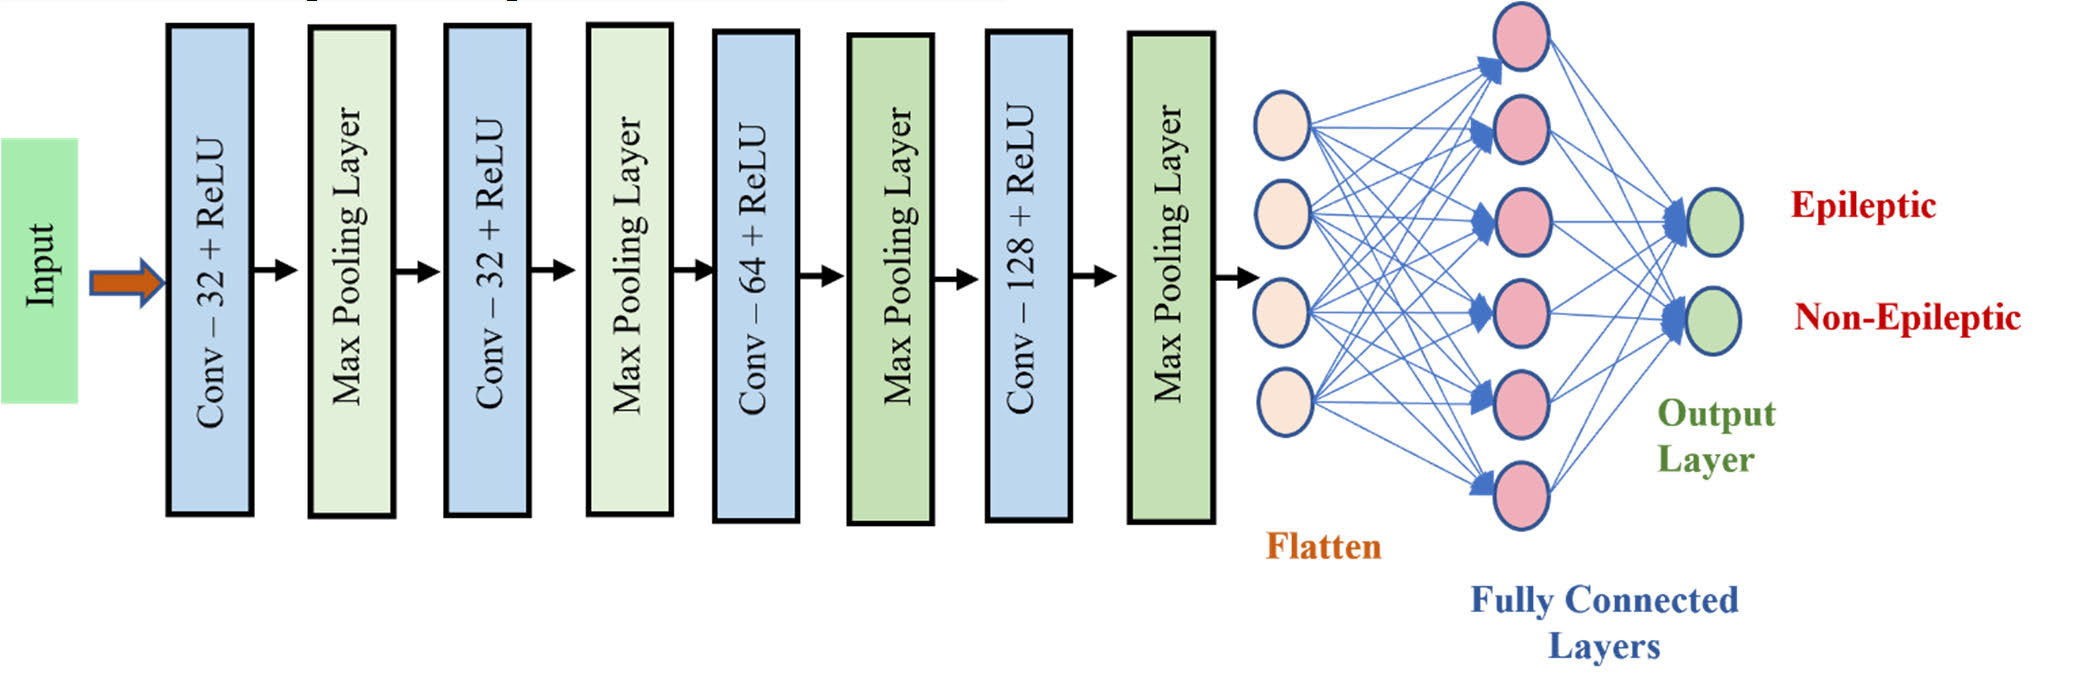
\includegraphics[width=1\linewidth]{Images/Figure 4.png}
    \caption{CNN architecture of the proposed method.}
    \label{fig:CNN_Arch}
\end{figure}

\chapter{Performance Evaluation And Results}

To assess the performance of the proposed method in differentiating seizures and non-seizures, the following evaluation metrics were computed: Accuracy, Precision, Recall, F1-Score, Critical Success Index (CSI), Matthews Correlation Coefficient (MCC), and Cohen's Kappa. Their mathematical definitions are given below:

\begin{equation}
\text{Accuracy} = \frac{TP + TN}{TP + TN + FP + FN}
\end{equation}

\begin{equation}
\text{Precision} = \frac{TP}{TP + FP}
\end{equation}

\begin{equation}
\text{Recall} = \frac{TP}{TP + FN}
\end{equation}

\begin{equation}
\text{F1-Score} = 2 \cdot \frac{\text{Precision} \cdot \text{Recall}}{\text{Precision} + \text{Recall}}
\end{equation}

\begin{equation}
\text{CSI} = \frac{TP}{TP + FN + FP}
\end{equation}

\begin{equation}
\text{MCC} = \frac{TP \cdot TN - FP \cdot FN}{\sqrt{(TP + FP)(TP + FN)(TN + FP)(TN + FN)}}
\end{equation}

\begin{equation}
\kappa = \frac{P_o - P_e}{1 - P_e}
\end{equation}

Where:  
\begin{itemize}
    \item $TP$ = True Positive (correctly predicted seizures)  
    \item $TN$ = True Negative (correctly predicted non-seizures)  
    \item $FP$ = False Positive (non-seizures misclassified as seizures, Type I error)  
    \item $FN$ = False Negative (seizures misclassified as non-seizures, Type II error)  
    \item $P_o$ = Observed agreement  
    \item $P_e$ = Expected agreement  
\end{itemize}




\section{Confusion Matrix}

The key evaluation metrics—accuracy, precision, sensitivity (recall), and specificity—were obtained from the confusion matrix. Figure~\ref{fig:confusion} presents the confusion matrices for the four classifiers, illustrating the distribution of true positives (TP), true negatives (TN), false positives (FP), and false negatives (FN). This visualization provides deeper insight into each model’s classification behavior beyond aggregated performance metrics.  

The results indicate distinct performance patterns across classifiers:  

\begin{itemize}
    \item \textbf{XGBoost (Figure 4.1 a):} Misclassified 10 non-epileptic instances as epileptic and 47 epileptic instances as non-epileptic.  
    \item \textbf{TabNet (Figure 4.1 b):} Exhibited a higher error rate, with 20 non-epileptic instances misclassified as epileptic and 75 epileptic instances as non-epileptic.  
    \item \textbf{Random Forest (Figure 4.1 c):} Misclassified 21 non-epileptic instances as epileptic and 26 epileptic instances as non-epileptic.  
    \item \textbf{1D-CNN (Figure 4.1 d):} Produced fewer errors, misclassifying 18 non-epileptic instances as epileptic and 9 epileptic instances as non-epileptic.  
\end{itemize}

These results provide valuable insights into classifier strengths and limitations. The TabNet classifier struggled the most, particularly in correctly identifying epileptic cases, making it less reliable for seizure detection. XGBoost and Random Forest showed moderate performance but still exhibited a significant number of false negatives, which is critical in medical applications. In contrast, the 1D-CNN model achieved the best balance, with relatively fewer misclassifications, suggesting its stronger ability to distinguish epileptic from non-epileptic signals.

\begin{figure}[htbp]
    \centering
    \subfloat[]{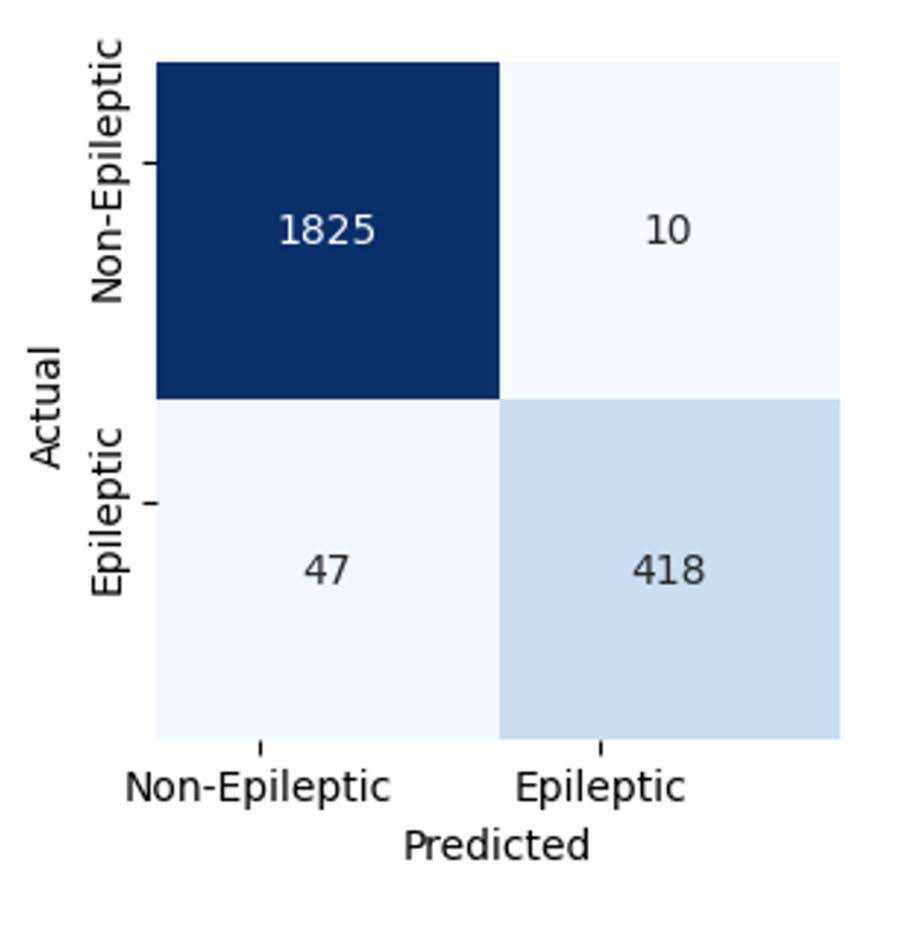
\includegraphics[width=0.45\linewidth]{Images/Figure 5a.png}} 
    \hfill
    \subfloat[]{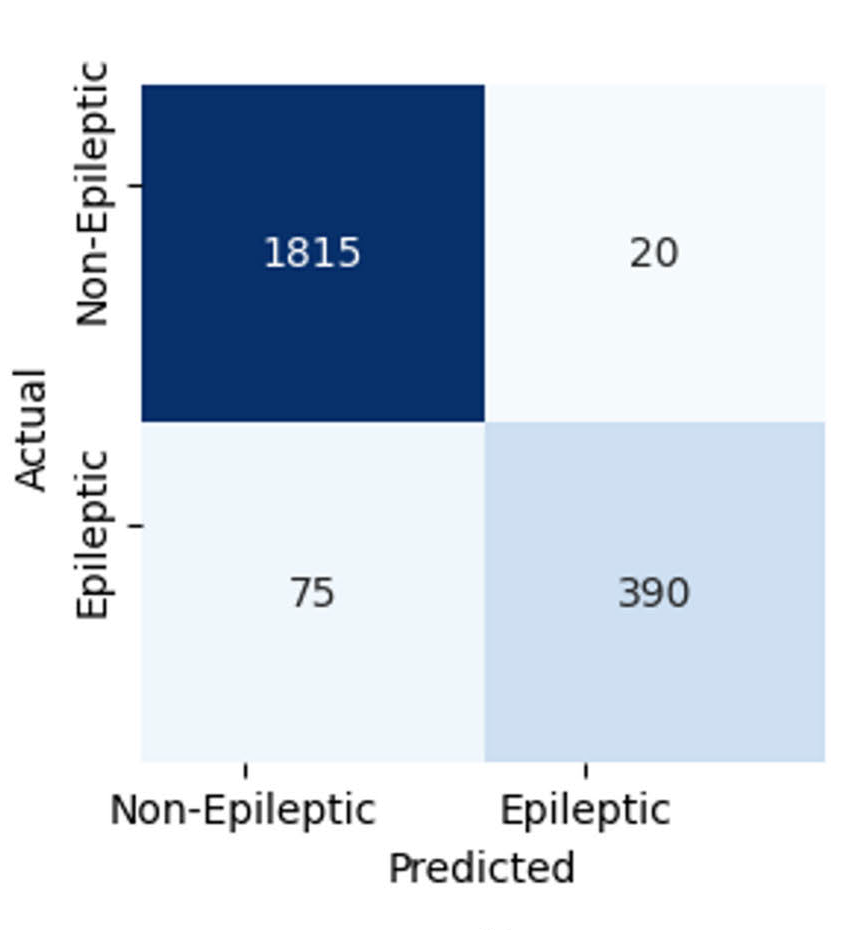
\includegraphics[width=0.45\linewidth]{Images/Figure 5b.png}} \\[1ex]
    \subfloat[]{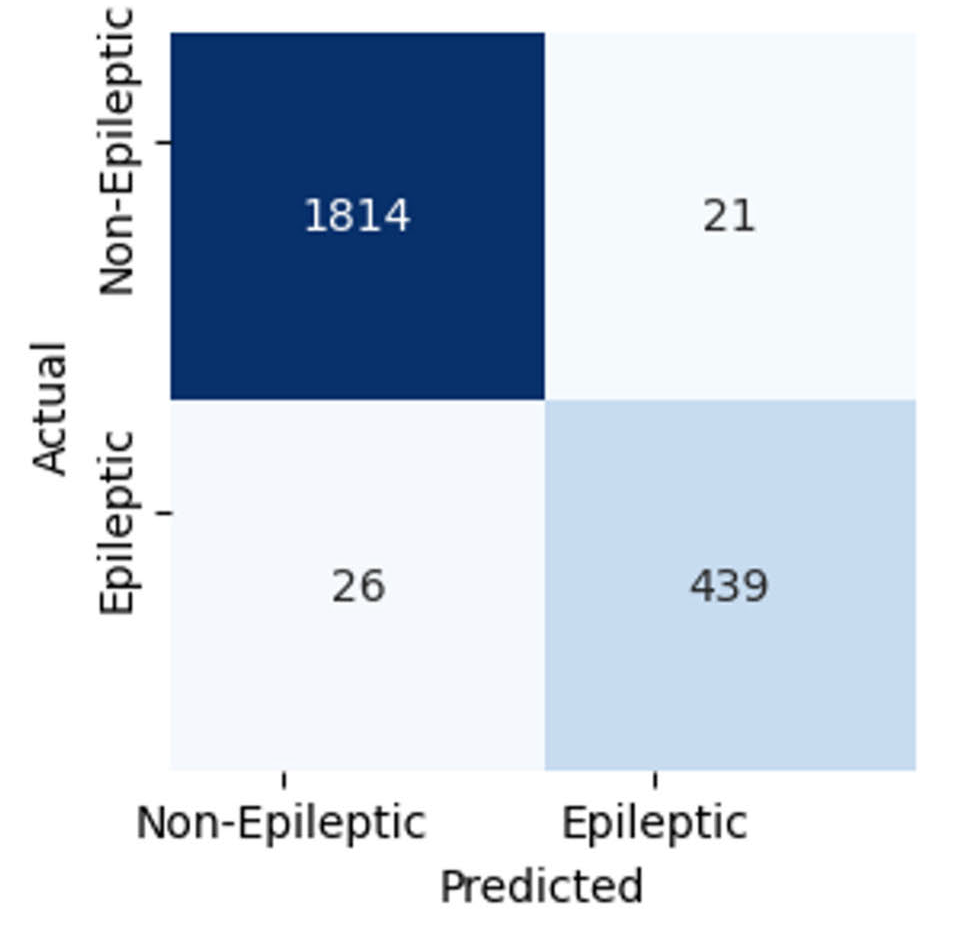
\includegraphics[width=0.45\linewidth]{Images/Figure 5c.png}} 
    \hfill
    \subfloat[]{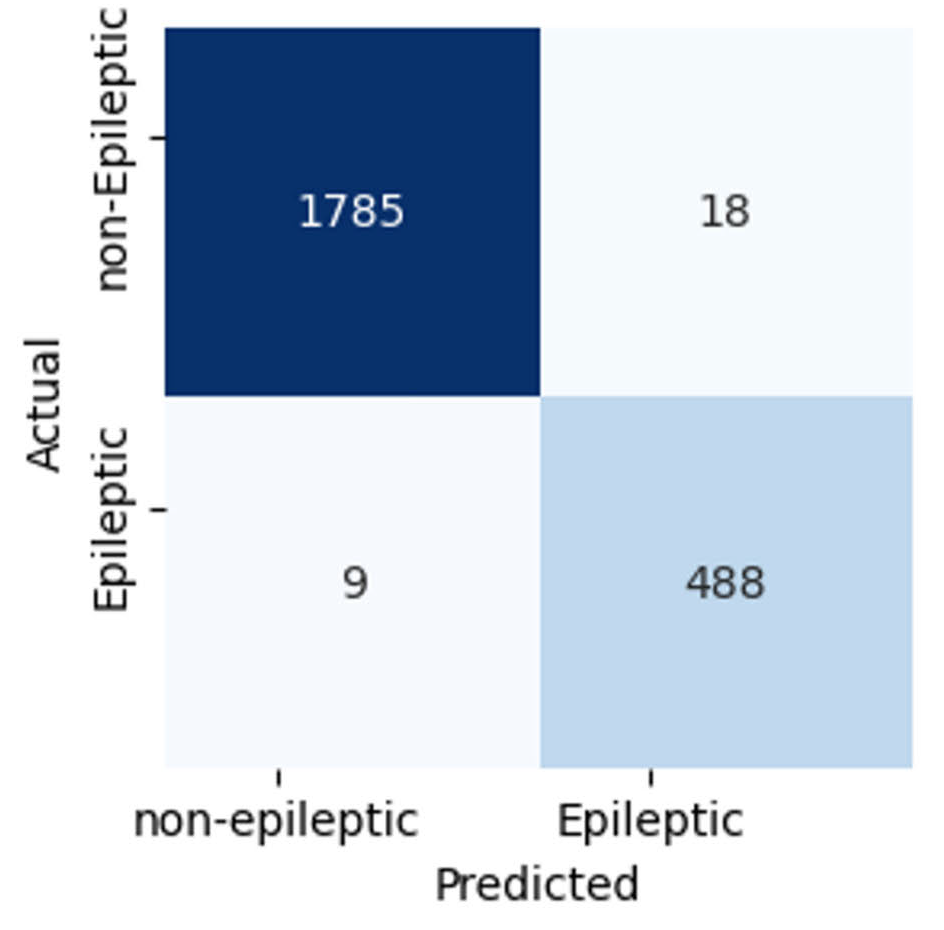
\includegraphics[width=0.45\linewidth]{Images/Figure 5d.png}}
    \caption{Confusion matrices for the classifiers: (a) XGBoost, (b) TabNet, (c) Random Forest, (d) 1D-CNN.}
    \label{fig:confusion}
\end{figure}



\section{ROC-AUC Curve}
The Receiver Operating Characteristic Area Under the Curve (ROC AUC) is a metric used to assess the performance of a classification model, mainly in binary class classification. It is a graphical representation between sensitivity (true positive rate) and specificity (true negative rate) across various threshold settings.


The ROC curve plots the true positive rate against the false positive rate, whereas AUC is the area under the ROC curve. In FIGURE 6, (a), (b), (c), and (d) have the AUC values of 0.997, 0.98, 1.00, and 0.98, respectively, which indicate that a has the AUC value of 0.997 and c has an AUC value of 1.00 which represents those proposed approaches reflects the perfect discrimination.



\begin{figure}[htbp]
    \centering
    \subfloat[]{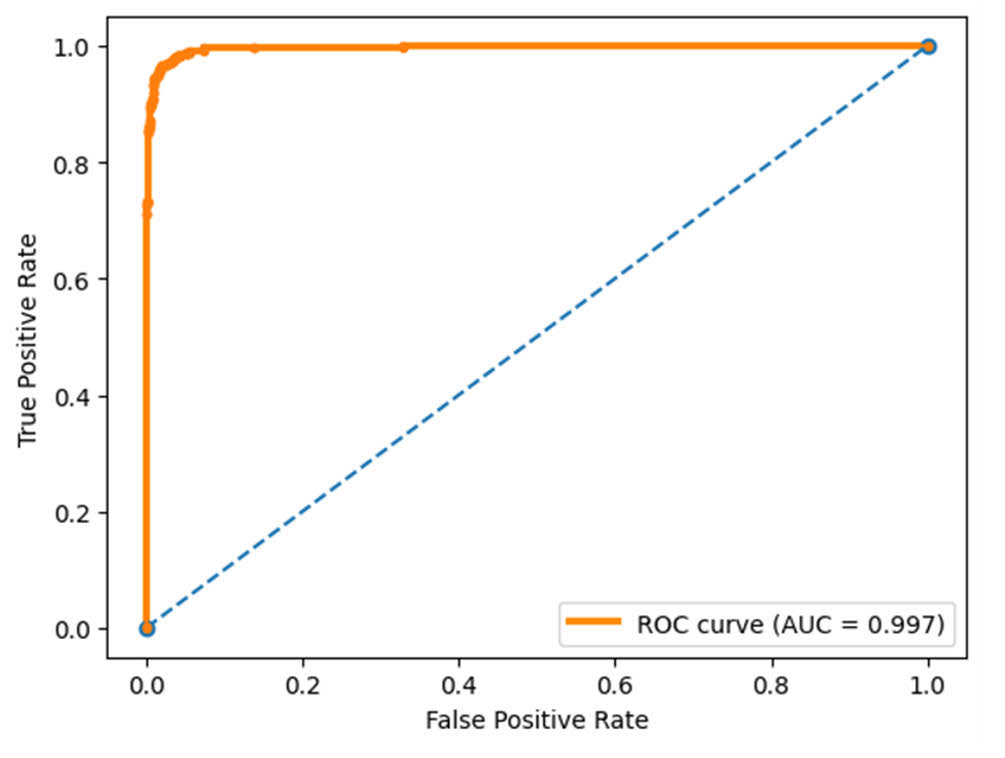
\includegraphics[width=0.45\linewidth]{Images/Figure 6 a.png}} 
    \hfill
    \subfloat[]{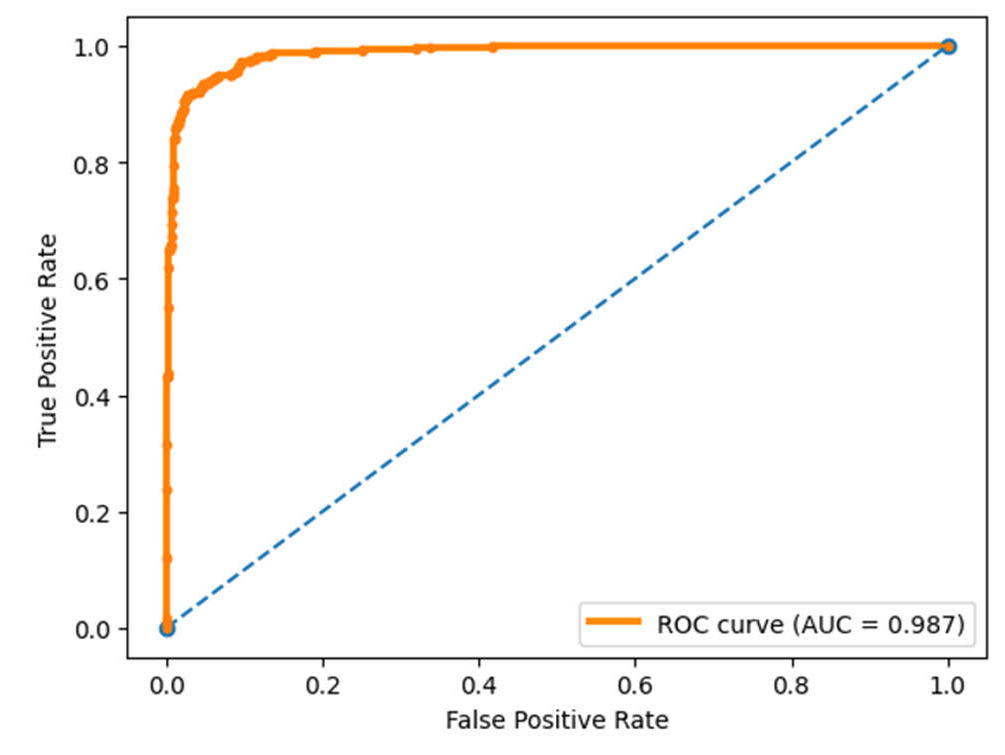
\includegraphics[width=0.45\linewidth]{Images/Figure 6 b.png}} \\[1ex]
    \subfloat[]{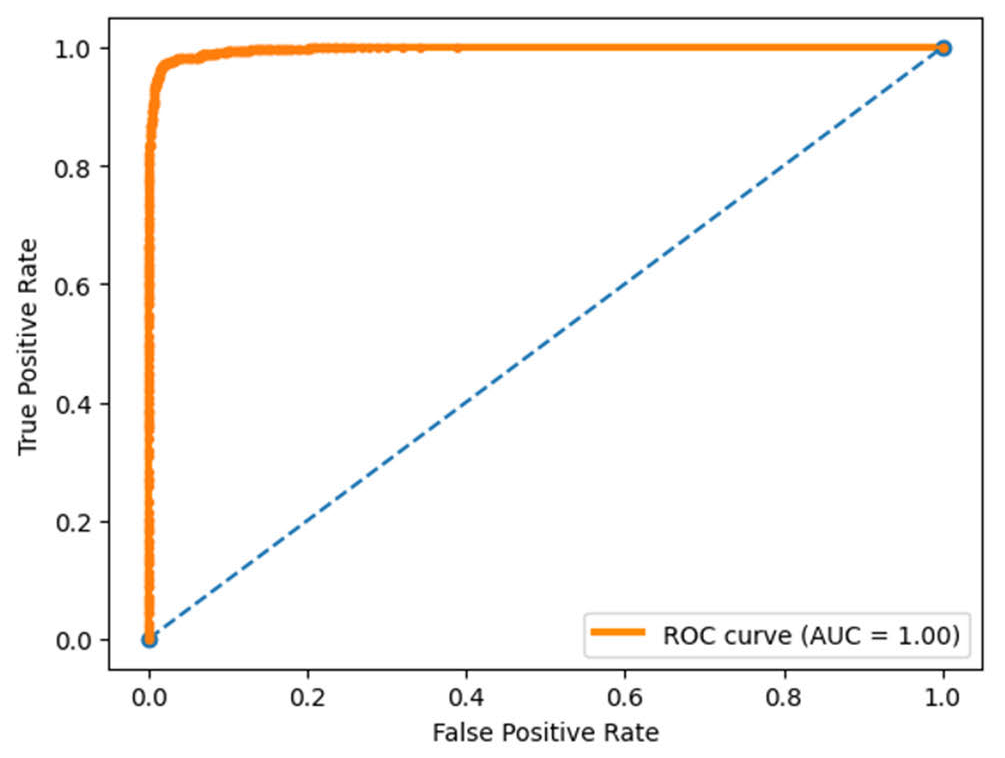
\includegraphics[width=0.45\linewidth]{Images/Figure 6 c.png}} 
    \hfill
    \subfloat[]{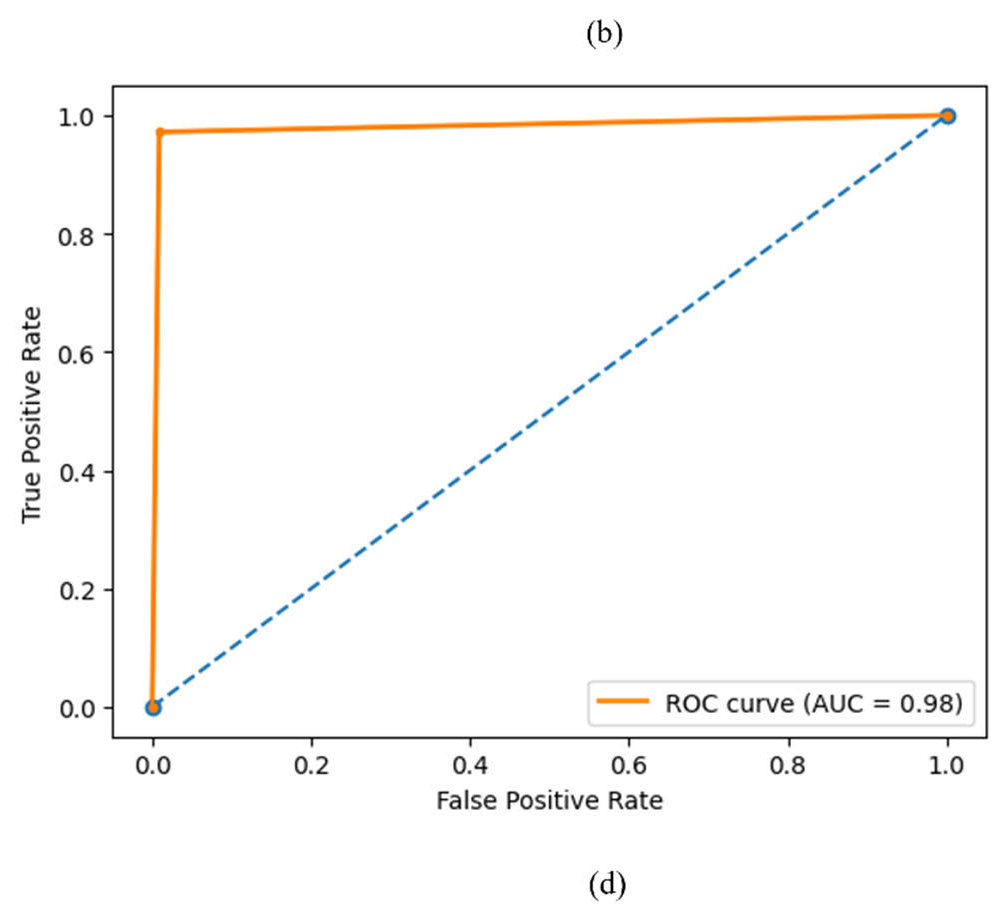
\includegraphics[width=0.45\linewidth]{Images/Figure 6 d.png}}
    \caption{ROC-AUC curve of four classifiers. (a) XGBoost, (b) TabNet, (c) Random Forest, and (d) CNN.}
    \label{fig:roc-auc}
\end{figure}

\section{CSI, MCC And Cohen's Kappa}
Additional metrics such as the Critical Success Index (CSI), Matthews Correlation Coefficient (MCC), and Cohen’s Kappa provided further insights into classifier performance. The XGBoost classifier achieved CSI, MCC, and Kappa scores of 0.88, 0.92, and 0.92, respectively. TabNet recorded 0.80, 0.86, and 0.86, while Random Forest achieved 0.90, 0.93, and 0.93. The 1D-CNN model outperformed the others with 0.94, 0.96, and 0.96, respectively.

Table 4.1 summarizes the experimental outcomes, including accuracies of 98\% (XGBoost), 96\% (TabNet), 98\% (Random Forest), and 99\% (1D-CNN). Weighted averages for Precision, Recall, and F1-score were used to address class imbalance, ensuring more representative evaluation. Validation loss values highlighted generalization performance: 0.06 for XGBoost, 0.13 for TabNet, and 0.02 for 1D-CNN, with the latter showing the best generalization.

Previous studies on epileptic seizure detection using EEG signals have reported promising results, often dependent on dataset characteristics. While several works improved 1D-CNN architectures with additional layers, our proposed 1D-CNN, using only convolutional, pooling, and classification layers, achieved comparable accuracy while standing out by delivering the highest sensitivity, precision, and recall.

\begin{table}[h!]
\centering
\caption{Weighted average values of the proposed method.}
\label{tab:results}
\begin{tabular}{|c|c|c|c|c|c|c|c|}
\hline
\textbf{Classifier} & \textbf{Accuracy} & \textbf{Precision} & \textbf{Recall} & \textbf{F1 Score} & \textbf{Kappa} & \textbf{MCC} & \textbf{CSI} \\ \hline
XGBoost      & 98 & 0.98 & 0.98 & 0.97 & 0.920 & 0.922 & 0.88 \\ \hline 
TabNet       & 96 & 0.96 & 0.96 & 0.96 & 0.86 & 0.86 & 0.80 \\ \hline
Random Forest & 98 & 0.98 & 0.98 & 0.98 & 0.93 & 0.93 & 0.90 \\ \hline
1D-CNN       & 99 & 0.99 & 0.99 & 0.99 & 0.96 & 0.96 & 0.94 \\ \hline
\end{tabular}
\end{table}


%%********************Chapter 5**********

%%********************Chapter 6**********
\chapter{Conclusion}
This research applied machine learning algorithms, including XGBoost, TabNet, and Random Forest, along with a tailored 1D-CNN architecture, to effectively classify epileptic seizures within EEG signals, with a deliberate focus on optimizing precision, recall, and F1-score in addition to accuracy. While many prior works have prioritized overall accuracy, our study emphasizes the importance of these complementary metrics in medical contexts, where correctly identifying positive seizure events and avoiding misclassification of non-seizure cases is vital for diagnosis and treatment. By introducing this comprehensive evaluation framework, we highlight an advancement over existing approaches, demonstrating that even with similar accuracies to previous studies, our models outperform them in precision, recall, and F1-score, offering more reliable clinical applicability. The experiments were conducted on the UCI epileptic seizure recognition dataset, which is derived from the Bonn University EEG database and provided in preprocessed \texttt{.csv} format. While this enabled efficient model training, it also introduces limitations, since reliance on pre-extracted data may exclude subtle but clinically significant EEG features, and the model’s performance ultimately depends on the quality of preprocessing. Furthermore, although careful parameter tuning allowed us to obtain strong results, unexplored regions of the feature space may hold further improvements, and the gap between controlled experimental settings and real-time seizure monitoring highlights the complexity of deploying such systems in practice. Challenges also remain due to the high variability of seizure patterns and patient-specific differences in EEG signals, which complicate the development of a universal detection framework. Addressing these challenges requires close collaboration among clinicians, neuroscientists, and machine learning experts. Future directions involve integrating multimodal physiological data sources such as EEG, ECG, and accelerometry to provide richer context, applying deep learning with domain adaptation techniques to improve generalization across patients, and adopting explainable AI methods to enhance interpretability and clinical trust. Together, these efforts point toward the development of more accurate, personalized, and accessible seizure detection systems that can support timely interventions and advance the state of the art in epilepsy care.








%%********************Chapter 7**********
\chapter{References}

\begin{enumerate}

\item A. Dogra, S. A. Dhondiyal, and D. S. Rana, ‘‘Epilepsy seizure
detection using optimised KNN algorithm based on EEG,’’ in Proc. Int. Conf. Advancement Technol. (ICONAT), Jan. 2023, pp. 1–6, doi:
10.1109/ICONAT57137.2023.10080847.

\item Y. Kaya, M. Uyar, R. Tekin, and S. Yıldırım, ‘‘1D-local binary pattern
based feature extraction for classification of epileptic EEG signals,’’ Appl.Math. Comput., vol. 243, pp. 209–219, Sep. 2014.

\item M. Mursalin, Y. Zhang, Y. Chen, and N. V. Chawla, ‘‘Automated epileptic seizure detection using improved correlation-based feature selection with random forest classifier,’’ Neurocomputing, vol. 241, pp. 204–214, Jun. 2017, doi: 10.1016/j.neucom.2017.02.053.

\item N. K. C. Pratiwi, I. Wijayanto, and Y. N. Fu’adah, ‘‘Performance analysis of an automated epilepsy seizure detection using EEG signals based on 1D-CNN approach,’’ in Proc. 2nd Int. Conf. Electron., 2022, pp. 265–277.

\item A. Abdelhameed and M. Bayoumi, ‘‘A deep learning approach for
automatic seizure detection in children with epilepsy,’’ Frontiers Comput. Neurosci., vol. 15, pp. 1–12, Apr. 2021, doi: 10.3389/fncom.2021. 650050.

\item I. Ahmad, X. Wang, D. Javeed, P. Kumar, O. W. Samuel, and S. Chen,
‘‘A hybrid deep learning approach for epileptic seizure detection in
EEG signals,’’ IEEE J. Biomed. Health Informat., pp. 1–12, 2023, doi:
10.1109/JBHI.2023.3265983.

\item Q.Wu and E. Fokoue, ‘‘Epileptic seizure recognition,’’ 2017. [Online]. Available: https://www.kaggle.com/datasets/harunshimanto/epilepticseizure-recognition, doi: 10.13140/RG.2.2.33336.03843.

\item T. Chen and C. Guestrin, ‘‘XGBoost: A scalable tree boosting system,’’ in Proc. 22nd ACM SIGKDD Int. Conf. Knowl. Discovery Data
Mining, San Francisco, CA, USA, Aug. 2016, pp. 785–794, doi:
10.1145/2939672.2939785.


\item  S. Ö. Arik and T. Pfister, ‘‘TabNet: Attentive interpretable tabular learning,’’ in Proc. AAAI Conf. Artif. Intell., vol. 35, no. 8, pp. 6679–6687, May 2021.

\end{enumerate}

\end{document}



se